\documentclass[../OAE-SPEC-MAIN.tex]{subfiles}

\title{Principles of Operation}

\begin{document}

\chapter{Principles of Operation}\label{sec:principles-of-operation}

\begin{marginfigure}	% Trim is left, bottom, right, top
\centering
   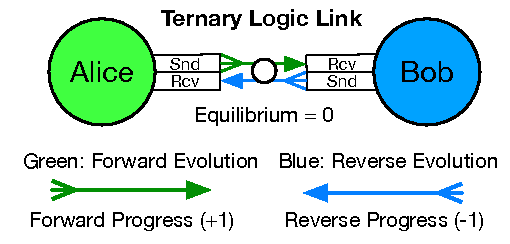
\includegraphics[width=1.15\textwidth]{./figures/ternary-link.pdf}
\caption{\centering Two \texttt{CELLs} and a \LINK with \emph{Conserved Quantities} (CQ) in dynamic equilibrium (Alternating Bit Protocol), epistricted with \href{https://en.wikipedia.org/wiki/Three-valued_logic}{Ternary Logic}}% \cite{threevaluedlogic2025}}
\label{fig:LINK}
\end{marginfigure}

This chapter defines the foundational principles that govern operation over \LINKs in Atomic Ethernet (\AE thernet). While traditional protocols prioritize throughput by maximizing raw bit rates, \AE thernet focuses on reversible, causally deterministic, and information-conserving communication. Rather than treating bandwidth as a fungible resource, \AE thernet embraces a model rooted in equilibrium, token transfer, and fixed-sized transactional units. This framing enables high reliability and high throughput data movement even in failure-prone environments, where every deviation from equilibrium is accounted for and correctable. We describe the architectural consequences of these choices, highlighting symmetry, liveness, and feedback-informed interaction.






\section{Symmetric Reversibility}

At the heart of Atomic Ethernet lies a symmetric, reversible link protocol, governed by deterministic state machines operating on both ends of a point-to-point connection. Together, these machines co-create a unified, bidirectional construct called a \LINK. \LINKs are not merely a passive channel, but an active agent with its own \textit{failure domain}, \textit{causal boundaries}, and defined \textit{error recovery semantics}.

A \LINK is thus a joint stateful system. Both peers (e.g., Alice and Bob) implement identical state machines that evolve synchronously via the exchange of fixed-size, causally significant tokens. These tokens encode both data and flow-control intent, and their transitions are mirrored on each end. There is no concept of master/slave. Either side may assume the role of \texttt{INITIATOR} or \texttt{RESPONDER}, depending on who possesses the token.

\begin{highlightbox}[Definitions]
\textbf{symmetric}: each side executes the same logic, defined by the same transition rules, enabling fully mirrored behavior. No global sequencing is required beyond token ownership.

\textbf{reversible}: for every operation on the link, there exists a logically defined inverse that restores the prior state.
\end{highlightbox}

Together, a \texttt{symmetric}, \texttt{reversible} protocol enables new guarantees on the network:
\begin{itemize}
\item Partial transactions can be aborted cleanly, returning to an equilibrium where no partial, unconfirmed state is leaked on either side.

\item Errors (e.g., bit flips, packet loss) can be rolled back without corrupting state.

\item All token transfers are atomic: they either complete fully or leave the system unchanged.
\end{itemize}

These properties allow \LINKs to resume normal operation even in the presence of transient failures. No global reset is needed; instead, local error recovery and rebalancing maintain the equilibrium between peers.

This symmetry and reversibility simplify correctness proofs, enable formal verification of protocol behavior, and provide a foundation for constructing reliable distributed systems from fundamentally unreliable components.


\subsection*{Physics is Time-Reversible}

Traditional networking systems are rooted in a \emph{Forward-In-Time-Only (FITO)} model--a consequence of human cognition and the constraints of classical computation. This FITO mindset leads to systems that rely on:
\begin{description}
\item[Preemption and Speculative Execution:]
Traditional systems often rely on speculative steps that assume future success, executing tasks before their prerequisites have fully resolved. When these guesses fail, the system must backtrack or retry. This introduces inefficiencies, side effects, and non-determinism. This speculative mindset is a direct byproduct of FITO thinking: always pushing forward, and retrying on failure.

\item[Halting and Sleep States:]
Mechanisms like halting, pausing, and sleeping (e.g., the Sleeping Beauty problem) reflect our inability to carry forward context across time. A container, for instance, may be restarted by Kubernetes without memory of its past states--like Rip van Winkle waking with no recollection of the world he once knew. This statelessness forces systems to infer or rehydrate their place in the world, often incorrectly.

\item[Retry Loops and Stuttering:]
When systems fail to complete an operation, the default response is to try again, often without understanding the cause of failure. This leads to stuttering behaviors: repeated attempts that may succeed eventually, but with no guarantee of consistency or progress. These retry loops clog the network, waste energy, and complicate reasoning. Worse, they mask latent failures and blur accountability.
\end{description}

But nature itself is reversible. When we model computation and communication the same way, we open up new possibilities: conserved quantities, reversible transactions, and memory-ful systems that avoid redundant restarts. Instead of containers that forget and retry blindly, \LINKs can maintain identity and progress symmetrically.

Within the link, we distinguish between \textbf{entanglement} (externally visible state) and \textbf{intanglement} (internally distinguishable state). Even when a system appears symmetric from the outside, internal roles can be differentiated. For example, a two bit counter incremented on each token exchange can ensure that Alice always sees odd tokens and Bob sees even counts, allowing each side to infer causality without global coordination.

This model reinterprets what coherence means on the wire. Prior attempts like Homa (at L3) or Aeron (at L4) focus on throughput and tail latency, but fail to establish reliable pairing of messages. \AE thernet instead solves the pairing problem at the layer it was created: Ethernet.



\subsection*{Temporal Intimacy and Message Coherence}

Symmetric reversibility permits a form of \emph{temporal intimacy}: a tight binding between request and response that emerges not from round-trip timers or speculative sprays, but from the causal loop of token exchange. This cannot be emulated at higher layers; it is a property of the \LINK itself.

Approaches like Amazon’s SRD (Scalable Reliable Datagram) scatter packets across paths to reduce jitter, and RoCE uses Priority Flow Control (PFC) to simulate backpressure, but both ultimately introduce complexity and failure modes (e.g., head-of-line blocking, incast microbursts, silent corruption) that are sidestepped entirely with a conserved, reversible link protocol.

Instead of relying on retry logic, timeout windows, or routing indirection, \AE thernet builds coherence into the wire. Every token is a conserved object: inserted, tracked, and retired without ambiguity. This enables applications to own and reason about their own network semantics — spanning trees, message lifetimes, and all.

This is not just a transport improvement. It is a paradigm shift, replacing FITO assumptions with a model that aligns closer to physics, and gives us new tools to reason about responsibility, identity, and truth in distributed systems.









\section{Interactions, not Bandwidth}

Traditional networks treat bandwidth as a fungible resource; Like a pipe to be filled as much and as fast as possible. Success is measured in utilization, and failure in dropped packets. In contrast, \AE thernet redefines communication as a series of causal interactions between peers, where each exchange has semantic weight and is governed by \LINK state machines.

In this model, throughput is an emergent property of sustained, reversible token exchanges — not burst transmission. Initiators flow frames toward responders without waiting, and responders flow responses back in kind. The rate of progress is governed not by the raw link speed, but by the rate of acknowledged interaction. This change in framing brings several practical consequences:
\begin{itemize}
\item \textbf{Stable Congestion Behavior}: Systems built on causal flow control naturally avoid head-of-line blocking and buffer overflows, especially under sustained high load.
\item \textbf{Implicit Clock Recovery}: Each interaction provides timing and synchronization cues, enabling robust clock alignment without separate timing channels.
\item \textbf{Minimized Latency Variance}: Because there are no speculative transmissions, queuing and jitter are dramatically reduced, even under full load.
\item \textbf{Atomic Forward Progress}: A transfer either completes causally or is fully rolled back, preserving global consistency without the need for speculative multi-path packet spraying.
\end{itemize}


\subsection{Hidden cost of Bandwidth-First}

Raw, one-way Bandwidth metrics alone fail to account for the crucial aspect of round-trip reliability--the guaranteed and verifiable transfer of knowledge between nodes. Such guarantees require explicit handshakes by the hardware to properly transfer ownership and responsibility of each packet with the lowest possible latency. Without these mechanisms, software interfaces cannot trust intermediate nodes to handle their knowledge responsibly.

In contrast, bandwidth-maximizing designs focus primarily on pushing bit streams at peak throughput. Their impressive bandwidth benchmarks are typically achieved by sending large, uninterrupted byte sequences that minimize overhead. These systems are engineered to drop packets during congestion, prioritizing throughput numbers over the integrity or reliability of tokens.

\begin{marginfigure}
  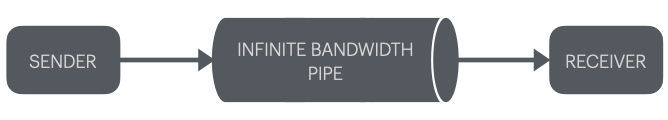
\includegraphics[width=\linewidth]{./figures/InfiniteBandwidthPipe.png}
  \caption{A infinite bandwidth pipe with packet loss can still limit throughput of TCP flows.}
  \label{fig:infinite_bandwidth}
\end{marginfigure}

\marginpar{
  \[
    \text{BW} = \frac{\text{MSS}}{\text{RTT}} \cdot \frac{C}{\sqrt{p}}
  \]
  \scriptsize
  \textbf{MSS}: max segment size \\
  \textbf{RTT}: round-trip time \\
  \textbf{C}: constant (1.22) \\
  \textbf{p}: packet loss probability
}

Consider a lossy link with infinite bandwidth, as illustrated in Figure~\ref{fig:infinite_bandwidth}. In this hypothetical, the bottleneck is not raw capacity but the twin constraints of latency and packet loss. Since TCP relies on acknowledgments to regulate its sending rate, the time it takes to complete a round trip --RTT -- becomes a limiting factor on throughput. As shown by the Mathis equation\cite{mathis1997}, throughput degrades proportionally to the inverse of RTT and the square root of the loss probability. In such regimes, increasing bandwidth alone does not improve performance; if anything, the absence of reliable round-trip feedback renders the network incapable of sustaining high-throughput flows. Even in a system of perfect raw transmission capacity, epistemic uncertainty introduced by loss and latency can strangle performance. Round trips are essential to any communication that requires certainty, ordering, or acknowledgment.

In practical networks where congestion is a real and dynamic force, TCP flows must adapt their behavior to avoid collapse. This adaptation is governed by Additive Increase/Multiplicative Decrease (AIMD) -- a deceptively simple algorithm that allows each sender to probe the available capacity of the network while reacting swiftly to congestion signals. Each flow increases its sending window linearly over time, but upon detecting loss (interpreted as a sign of congestion), it slashes the rate multiplicatively. This feedback loop produces a sawtooth pattern in throughput, enabling multiple flows to converge to a fair, stable sharing of the underlying path. Crucially, AIMD is fully decentralized and stateless beyond the endpoints. Yet, this elegant self-regulation only functions when loss reflects congestion, and when RTT remains a trustworthy signal of delay. In networks where loss is stochastic or induced by buffer mismanagement, AIMD underperforms or misbehaves \cite{Gettys2012} -- but in its ideal regime, it is a marvel of distributed equilibrium: each sender, optimizing selfishly, contributes to global stability.

Packet loss and network congestion represent more than inefficiency, they threaten the epistemic state of distributed systems. When a packet is dropped due to congestion, the information it carried vanishes completely, erasing knowledge of the event it represented. This loss isn't just temporary. It's fundamental and irreversible. Without this information, no node or application can know if the packet is coming late, or not at all. Exactly-once semantics rely entirely upon preserving and transferring this epistemic state across nodes. Failures in handling epistemic state leads to inconsistency and grey failures\sidenote{Grey failures represent a class of failure where events are partially known or suspected, but never fully provable}. Thus, the hidden peril of the bandwidth-first approach emerges clearly: by optimizing purely for throughput at the expense of reliable delivery, one risks catastrophic losses in epistemic certainty, fundamentally undermining the correctness and reliability of distributed computation.


\subsection{Are Acknowledgments Expensive? Not Anymore}

Traditional wisdom paints acknowledgments as throughput killers: in stop-and-wait protocols, the sender halts until it receives confirmation before transmitting again. But in modern Ethernet--particularly at 100\,Gbps over short links--this notion is obsolete. In fact, acknowledgments can be issued and received \emph{in-flight}, with virtually no cost to throughput.

Let’s examine why.

\begin{itemize}
  \item \textbf{Frame size (including overhead)}:
  \[
  64\text{B} + 8\text{B}\,(\text{preamble}) + 12\text{B}\,(\text{IPG}) = 84\,\text{bytes} = 672\,\text{bits}
  \]
  \item \textbf{Transmit time at 100 Gbps}:
  \[
  T_{\text{tx}} = \frac{672\ \text{bits}}{100 \times 10^9} = 6.72\ \text{ns}
  \]
  \item \textbf{Propagation speed}: \(2 \times 10^8\) m/s (5 ns per meter)
  \[
  \text{Length on wire} = T_{\text{tx}} \cdot v = 6.72\,\text{ns} \times 2 \times 10^8\ \text{m/s} = 1.344\ \text{m}
  \]
\end{itemize}
\vspace{1em}

\textbf{That means the entire frame is over a meter long on the wire--longer than many physical links.} For links under this length, the first bits of the frame can arrive at the receiver before the last bits have even left the sender.

This framing leads to a surprising result: on short links, round-trip time (RTT) is often shorter than transmission time. The table below compares these values and shows utilization (\( U = \frac{T_{\text{tx}}}{T_{\text{tx}} + \text{RTT}} \)):

\begin{center}
\begin{tabular}{@{}lccc@{}}
\toprule
Cable Length & RTT (ns) & $T_{\text{tx}}$ (ns) & Utilization ($U$) \\
\midrule
10 m  & 102.4  & 6.72   & 6.16\% \\
1 m   & 12.4   & 6.72   & 35.14\% \\
10 cm & 3.4    & 6.72   & 66.40\% \\
1 cm  & 2.5    & 6.72   & 72.88\% \\
\bottomrule
\end{tabular}
\end{center}

The shorter the link, the more transmission dominates RTT, and the higher the achievable utilization—even with a per-packet acknowledgment model.

\subsection{\AE thernet: Circulating Snakes}

In this model, each packet and its response form a closed-loop interaction: a reversible token with a forward and return path. Like a snake on a track, the packet’s body spans the link, and the acknowledgment follows behind, curling the path into a circuit of semantic closure. The only idle space is the inter-packet gap between snakes.

\begin{marginfigure}
  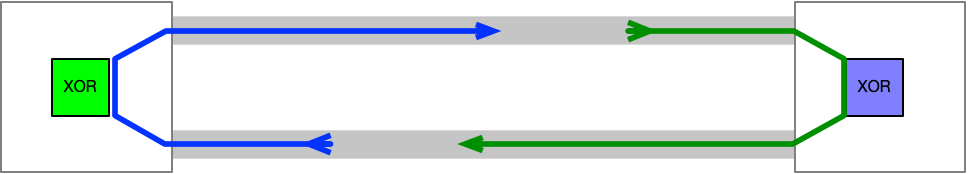
\includegraphics[width=\linewidth]{./figures/SNAKE_dualframe.png}
  \caption{In short links, a 64-byte packet spans the wire, with its acknowledgment returning before transmission completes—forming a circulating snake.}
\end{marginfigure}

This has profound implications:

\begin{itemize}
  \item \textbf{Acknowledgments are in-flight, not blocking}.
  \item \textbf{Causality is enforced at hardware speed}.
  \item \textbf{Utilization is limited only by the spacing between interactions—not protocol overhead}.
\end{itemize}

There’s no stop-and-wait. No idle windows. No speculative retries. Every token sent is causally resolved or rolled back. This transforms acknowledgments from a performance tax into a foundational mechanism for maintaining epistemic certainty.

This leads to a key insight: acknowledgments don’t require idle time. They can be:

\begin{itemize}
  \item \textbf{Embedded or piggybacked} in return frames,
  \item \textbf{Pipelined} using snakes as carriers,
  \item \textbf{Issued in parallel} with frame reception.
\end{itemize}

Modern Ethernet resembles a conveyor belt more than a stoplight. Multiple frames are in motion, bidirectionally, all the time. With proper credit-based flow control, there’s no need to wait for a response before initiating the next action.

Acknowledgments--once considered expensive--are now cheap, even free, on modern high-speed links. As frames stretch out physically and RTT shrinks, acknowledgment can arrive before the sender finishes transmission. Add to this the amortization effects of jumbo frames and the elegance of pipelined protocols, and the old “stop-and-wait” bottleneck dissolves.








\section{Fixed size Slots, Perfect Information Feedback}

\AE thernet operates exclusively on fixed-size records, or \emph{slots}, ensuring every transaction carries a known, bounded amount of entropy. This constraint, far from limiting expressiveness, unlocks a powerful class of deterministic behaviors aligned with the structure of digital hardware and the limits of information theory. Each transaction transfers exactly one slot: a fixed-length, self-contained unit of data and control.

Because slots are of known and equal size, \textbf{flow control is dramatically simplified}. This ensures that the sender knows exactly how much information is in flight, and the receiver can verify completeness without ambiguity. There is no need to infer transfer boundaries, negotiate variable lengths, or guess at incomplete frames. Every interaction is atomic and unambiguous. The result is a link state that evolves in predictable, stepwise increments.

\begin{highlightbox}[Definitions]
\begin{itemize}
\item \textbf{Shannon Slots}, the logical atomic units of information maintained in the protocol state machine (typically within FPGA registers).
\item \textbf{Wire Slots}, the physical representation of a slot as it is serialized across the wire.
\end{itemize}
\end{highlightbox}


The transition from Shannon Slot to Wire Slot is a fixed-length encoding operation — deterministic, invertible, and clock-aligned. Timing closure in the FPGA limits the frequency at which these slots can be emitted or consumed. However, because the slot size is constant and interaction is feedback-governed, the system avoids speculative overrun and maintains perfect pacing even at high utilization.

\AE thernet treats \textbf{Shannon slots as conserved quantities}. Each slot represents an indivisible unit of knowledge. Slots are never silently dropped, corrupted, or left in undefined states. This conservation principle draws a key distinction from best-effort packet-switched networks, where data loss is expected and recovery is probabilistic. In \AE thernet, every Shannon slot is not merely a container of bits, but a semantic object with causal responsibility.

\AE thernet is fully \emph{reversible}; on any error the receiver can reverse the transfer of a token returning ownership, and return responsibility  for correct operation to the initiator  (e.g. Hardware Error, Protocol violation, Software Error or resource exhaustion error). 





%\section{From API to Bits-on-the-wire}

%\AE thernet introduces a fundamentally new substrate for reliable communication. Every transmission is atomic, reversible, and causally consistent. To application developers, this creates the illusion of an \textit{unbreakable network}, where transactions either succeed completely or fail without side effects.

%Yet to enable adoption, \AE thernet must integrate seamlessly with existing infrastructure. The compatibility boundary is the IP layer. Above this layer, applications continue to operate as before. Below it, \AE thernet provides a drop-in replacement for traditional Ethernet, unobservable by legacy systems, but dramatically more reliable in behavior.

%However, the true potential of \AE thernet lies beyond emulation. Its atomic transaction model enables a new class of guarantees -- deterministic delivery, fault-local reversibility, and programmable transport semantics -- that cannot be expressed in the traditional IP or TCP abstractions. To expose these capabilities to applications, a new vertically integrated stack is needed.

%This stack must:
%\begin{itemize}
%\item Extend from the API boundary (e.g., sockets, RPC, shared memory transport) down to the bits on the wire.
%\item Preserve atomicity and reversibility guarantees across all abstraction layers.
%\item Offer language-level semantics (e.g., async/await, futures, or transactions) that map directly to causal protocol operations.
%\end{itemize}

%In essence, \AE thernet is not just a new physical protocol. It is a new foundation for building distributed systems, one in which software and hardware speak the same language of atomic, bidirectional flow.

%New transaction guarantees can be offered to applications, but requires a entirely new networking stack from API to bits on the wire that propagates the same guarantees of atomicity and reversibility into the languages that application developers write code with.





\section{Imposition vs. Promise Networks}

At the heart of modern networking lies a fundamental architectural choice: whether communication is \textbf{imposed} or \textbf{promised}. This distinction shapes not just how data is transmitted, but whether it arrives usefully—or contributes to congestion.

\subsection*{Imposition Networks}

In an \emph{imposition network}, transmitters force their state onto the fabric, assuming the network will carry and deliver their packets.\sidenote{Classic Ethernet operates this way: a sender injects frames without guarantee of delivery.} If a switch is overloaded, a buffer is full, or a receiver is slow, frames are dropped silently. The network does not push back; the burden of recovery is delegated to higher layers like TCP, which react only after detecting loss.

This model works under light load and modest expectations, but under stress, it fails noisily. Without link-layer accountability, the sender has no idea how the network is coping—until it’s too late.

\subsection*{Promise Networks}

\emph{Promise networks} invert the flow of responsibility. Rather than pushing unilaterally, each agent advertises what it will accept, under clearly stated conditions. Transmission becomes a handshake, not a shove.

These networks are built on \textbf{contracts}: link-local credits, flow control, congestion notification, and explicit acceptance of responsibility.\sidenote{Technologies like InfiniBand, Fibre Channel, and CAN are promise networks by design.} Ethernet-based protocols such as RoCEv2 attempt to retrofit this model via Priority Flow Control (PFC), with mixed results.

\subsection*{Paired vs. Unpaired Traffic}

The difference between these network philosophies becomes clear when categorizing traffic:

\begin{description}
  \item[Paired (Acknowledged) Traffic] Every frame is matched by a return promise—an acknowledgment, a credit, or some confirmation that the receiver is ready. These packets carry not just data, but a commitment to deliver it reliably.
  \item[Unpaired (Blind) Traffic] Sent speculatively or in excess of what the receiver can accept, these packets consume bandwidth, saturate buffers, and are often dropped. They provide no assurance of delivery and may never be noticed by the receiver.
\end{description}

Promise networks emphasize paired traffic, ensuring that every transmitted bit contributes to mutual information.\marginnote{Unpaired frames do not increase entropy—they leave a correlation hole.} Imposition networks permit unpaired traffic to accumulate, especially under congestion, where it becomes noise—expensive, harmful, and avoidable.

\subsection*{The Congestion Pathology}

Unreliable links are not a solution to congestion, they are its amplifier. When loss is used as a congestion signal, it arrives \emph{late}: often one to three round-trip times after the overload has begun. Meanwhile, high-throughput endpoints may inject millions of unpaired frames, deepening the crisis.

\begin{quote}
\centering
\texttt{loss $\rightarrow$ retransmit $\rightarrow$ more traffic $\rightarrow$ more loss}
\end{quote}

This positive feedback loop turns instability into collapse.\sidenote{TCP's loss-based control is inherently reactive and lagging.} Attempts to band-aid the problem, like bufferbloat, only add latency and jitter. Head-of-line blocking, reordering, and recovery delays further degrade tail-latency guarantees.

\subsection*{Promised Traffic on \AE thernet}

At the core of \AE thernet’s reliability is a circulating token: a physical representation of promise and permission to transmit. Each token is issued by the receiver, and it embodies a credit of exactly one frame. A sender must possess a token to transmit; the token carries the data forward, then returns with its own embedded acknowledgment.

Tokens are not metaphors—they are \emph{entities} in the protocol: atomic, bounded, and verifiable. They circulate continuously between two state machines on either end of a link, forming a closed loop of accountability.

\begin{marginfigure}
\centering
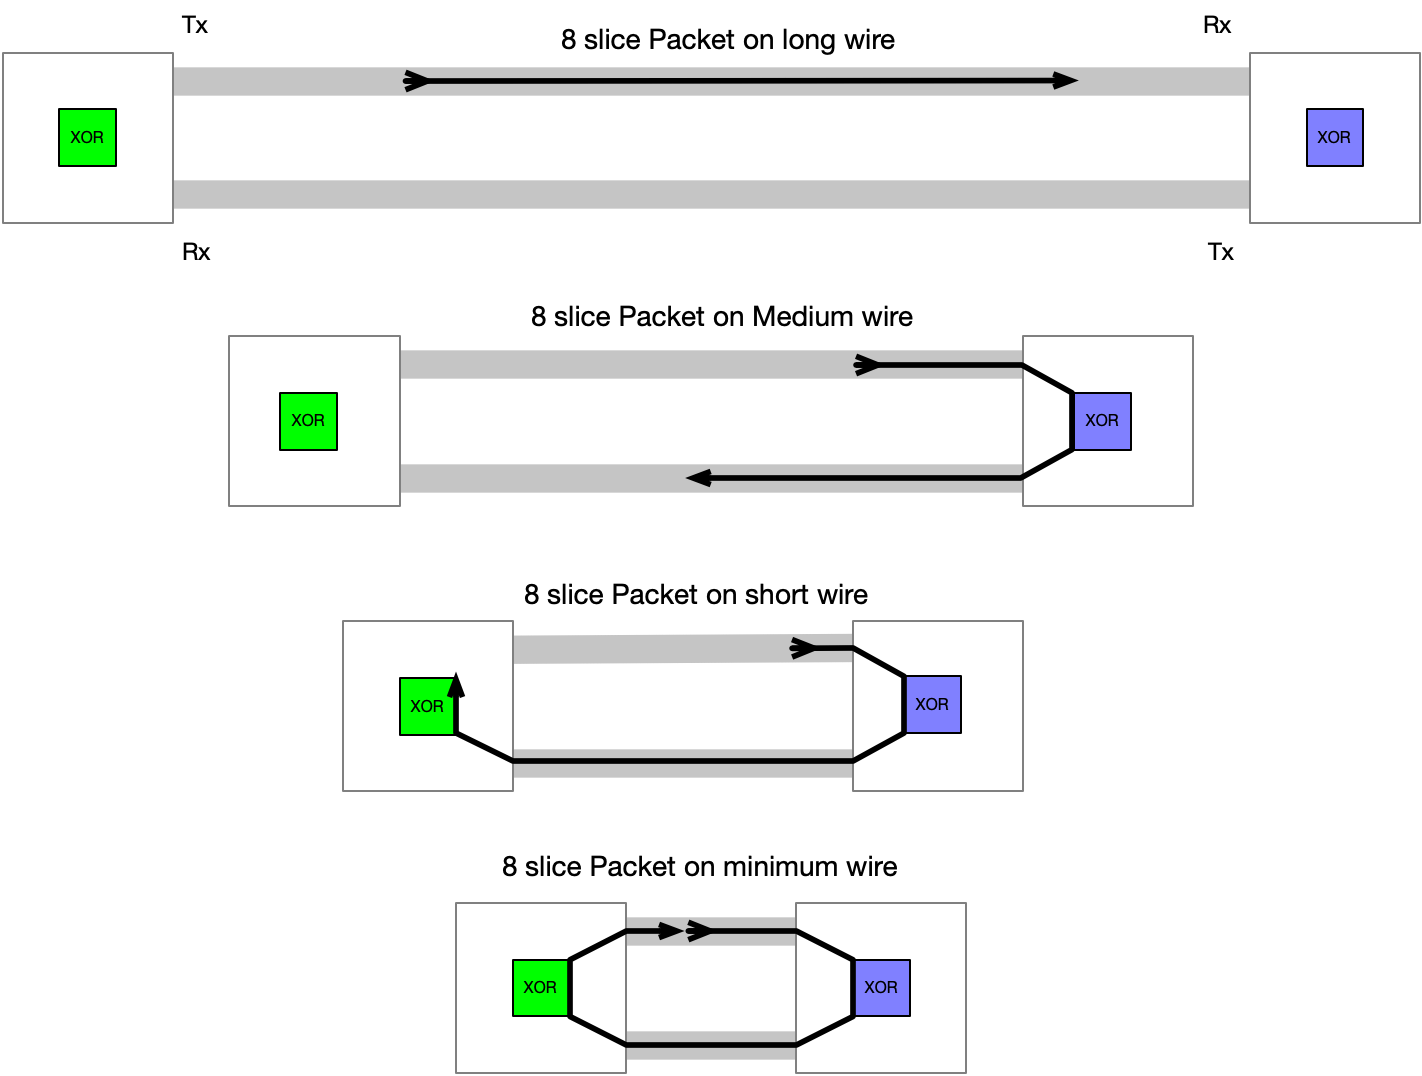
\includegraphics[width=\linewidth]{./figures/SNAKEs.png}
\caption{Each token carries data forward and acknowledgment back, ensuring pairing and fairness at the link level.}
\end{marginfigure}

Because a sender cannot outpace the receiver’s ability to consume and recycle tokens, congestion becomes \emph{visible} at the source as backpressure from the network. Transmission slows not due to dropped packets, but because tokens are withheld—the fabric communicates its limits by design, not through failure. This token-based link discipline gives rise to a new set of capabilities:

\begin{description}

  \item[Link-level feedback]  
  Feedback is embedded in the physics of the link. There is no guesswork, no need for loss-based heuristics. If tokens stop arriving, the sender knows immediately that the path is congested. All outstanding data is bounded by the number of tokens in flight, making buffer overflow and speculative retransmission impossible.

  \item[Lossless credit return]  
  Each token is both a permission and an acknowledgment: it grants authority to send and confirms receipt of the last transmission. This dual role eliminates the need for separate ACK channels and ensures all traffic is paired and meaningful. There is no such thing as an unacknowledged frame in \AE thernet.

  \item[Actionable ECN marks]  
  With loss removed as a congestion signal, Explicit Congestion Notification (ECN) becomes trustworthy. Tokens can be marked in-line when passing through congested nodes, then returned to the sender along their normal acknowledgment path. This allows for immediate, unambiguous congestion signaling with no packet loss and no guesswork.

  \item[Deterministic latency]  
  Because the number of tokens—and thus the number of outstanding frames—is bounded, queues are shallow and predictable. Latency is no longer subject to stochastic variation from contention and buffering. Determinism emerges naturally from the enforced pacing and bounded concurrency of the link.

  \item[Energy efficiency]  
  With no retransmissions, minimal buffering, and no speculative sending, energy is spent only on useful work. Tokens eliminate waste: every bit transmitted corresponds to a committed delivery. Hardware can be lean, buffers can be shallow, and network silicon can focus on forward progress, not recovery.

\end{description}

By grounding transmission in physical promises—tokens that carry both data and acknowledgement—\AE thernet transforms the network from an imposition fabric into a promise fabric. It closes the loop between sender and receiver at the lowest level, eliminating the uncertainty that drives modern congestion pathologies. Every packet delivered is not just seen—it is \emph{agreed upon}, exactly once.








\section{Exactly Once Delivery}

\subsection*{Best-Effort is not Good Enough}

Best-effort delivery means packets may be lost, reordered, duplicated, or delayed arbitrarily, and the network makes no guarantees beyond basic frame integrity. This was tolerable when applications lived on the same machine or within a few hops of each other and could tolerate latency spikes or re-transmissions. Today, however, large-scale systems depend on deterministic behavior:
\begin{itemize}
	\item \textbf{Distributed databases} depend on atomic commit, snapshot isolation, and causal ordering.
	\item \textbf{Control loops} in robotics and finance demand low-jitter, bounded-latency paths.
	\item \textbf{AI accelerators} and smartNICs coordinate at sub-microsecond time scales.
\end{itemize}
\vspace{1em}

Classical packet networks were never designed to guarantee \emph{reliability}.  From ALOHA to Ethernet, the assumptions of lossy media, finite buffers, and decentralized contention required higher layers to shoulder the burden of correctness.  Over time we have erected towering protocol stacks whose very purpose is to \emph{mask} loss, duplication, reordering, and delay.  Yet the mechanisms we depend upon--\textit{timeouts and retries}--carry hidden costs that threaten latency, availability, and correctness in ways subtle and profound.

Packets may vanish without a trace (loss), arrive multiple times (duplication), appear in bizarre permutations (reordering), or crawl through the network long after their sender has moved on (delay).  Physical phenomena such as bit errors, congestion, link flaps, and transient routing loops ensure that these pathologies are not edge cases but everyday realities.  The canonical wisdom \textemdash embodied in TCP, QUIC, and countless RPC frameworks \textemdash is to \emph{wait} for an acknowledgement and, failing that, \emph{retry}.  This simple recipe, however, is deceptively dangerous.

A \textbf{timeout} is an admission of ignorance: we do not know whether the message was lost or merely late.  We therefore \emph{speculate} by retransmitting.  Each additional round inflates network load, potentially exacerbating the congestion that caused the delay in the first place.  Worse, timeouts must be conservative---long enough to accommodate the \emph{long tail} of delays---or else false positives trigger needless work.  The tension between responsiveness and safety is irreconcilable: choose a short timeout and risk spurious resends, choose a long one and endure sluggish progress.


\subsection*{Timeout and Retries are the Root of All Evil}

Timeouts and retries (TAR) are a ubiquitous mechanism used in database systems, distributed systems, and network protocols to handle the inherent uncertainty of real-time and distributed environments. While they seem to be essential for providing fault tolerance and resilience, they can introduce significant anomalies, inefficiencies, and complexities into transaction systems, often leading to unintended consequences. This essay explores the inherent dangers and drawbacks of using timeouts and retries in distributed systems and databases, with references to transaction anomalies such as deadlocks, inconsistent states, and race conditions.

Distributed systems are inherently complex due to the need to coordinate and synchronize actions across multiple independent components. When an operation or transaction is executed in such systems, timeouts and retries often serve as a safety net. However, these mechanisms can create situations where the assumptions made about system state, consistency, and ordering are violated, leading to various anomalies.

\begin{description}

  \item[Deadlocks]  
  Retries can reintroduce or prolong circular dependencies in locking systems, especially under protocols like two-phase locking (2PL). A retried transaction may attempt to reacquire locks still held by other retried transactions, amplifying contention and risking system-wide stalling.

  \item[Inconsistent States]  
  Retrying a partially completed transaction without a full rollback can leave the system in an inconsistent state. Distributed updates that timeout mid-flight may result in divergent views across nodes, violating ACID guarantees.\sidenote{See \textcite{Lamport1978} and \textcite{Brewer2000}.}

  \item[Race Conditions]  
  Unsynchronized retries may overwrite concurrent updates, especially in eventually consistent systems.\sidenote{As discussed in \textcite{AmazonDynamo2007}.} If two transactions operate on the same key with conflicting logic, retries can lead to lost updates and read anomalies.

  \item[Resource Contention]  
  High retry rates can overwhelm limited resources--CPU, memory, or bandwidth--triggering more timeouts and creating a feedback loop of congestion. Sophisticated systems like \textcite{GoogleSpanner2012} mitigate this with controlled backoff and load-aware retry policies.

\end{description}


\subsection*{Exactly-Once Delivery: A Mirage}

Exactly-once semantics require that every message be delivered to the application \emph{once and only once}, despite failures.  In an asynchronous network with crash--stop faults, the famous FLP result shows consensus is unattainable without additional assumptions.  In practice, we settle for \emph{at--least--once} plus idempotent operations or \emph{at--most--once} with explicit application-level deduplication.  Timeouts and retries break the illusion of exactly-once by turning every uncertainty into a potential duplicate.

Under load, synchronized clients often hit the same timeout threshold, regenerating the same request and filling buffers anew.  This \emph{thundering herd} magnifies congestion, extends queueing delays, and forces still more timeouts--a positive feedback loop sometimes called a \emph{retry storm}.  Empirically, tail latencies inflate by orders of magnitude, and coordinated transactions miss their SLA windows. Eventually, upper layers declare failure, roll back work, or attempt compensating actions, further stressing the system.

\subsection*{Beyond Timeout and Retry}

The path to dependable systems begins not with coping mechanisms, but with structural guarantees. Instead of treating uncertainty as inevitable, we can engineer systems that reject ambiguity outright.

\begin{description}

  \item[Fail-Fast Links.]  
  Rather than tolerate silence, links should fail at the first sign of uncertainty. Inverting the logic of FLP, every ambiguity becomes a deliberate event—a trigger for rollback and recovery, not speculation. This model borrows from quantum triangle networks, where a third party observes and validates the transaction, ensuring that every failure is acknowledged and acted upon.

  \item[Verifiable Stacks.]  
  From API call to physical transmission, the full stack must be introspectable and enforce ownership, accountability, and intent. Every packet is a commitment; every bit must trace back to its origin. Only then can distributed systems enforce end-to-end responsibility.

  \item[Structural Backpressure.]  
  Congestion control must be native to the fabric, not bolted on. Credit-based protocols provide bounded buffers and network-level flow control, ensuring packets are never dropped due to oversubscription. The sender sees congestion as feedback, not failure.

  \item[Deterministic Delivery.]  
  In a truly reliable system, no packet is ever "lost"—it is either delivered or explicitly rejected. Conservation is paramount: every packet must be accounted for, even in failure. The sender must know, with certainty, the fate of every transaction.

\end{description}

We cannot build certainty atop silence. Timeout and retry are holdovers from a more forgiving era, where best-effort sufficed and correctness was the domain of upper layers. But at hyperscale, correctness must begin at the wire. Only by embedding reliability into the fabric—structurally, verifiably, and deterministically—can we create systems that are not only fast, but fundamentally sound.

Together, these four pillars—fail-fast semantics, verifiable responsibility, built-in backpressure, and packet conservation—form the basis for true exactly-once delivery. They eliminate ambiguity not through speculation, but through structure. When the network itself guarantees delivery, rejection, and accountability, the illusion of exactly-once becomes a reality. Not probabilistic. Not eventual. But provable.







\section{Beyond One-Way Counting Protocols}
Current network protocols predominantly rely on monotonically increasing sequence numbers to track packet delivery and ordering. This paper presents a fundamental critique of this approach, particularly focusing on TCP's one-way counting mechanism, and proposes an alternative framework based on conserved quantities (CQ). We demonstrate how a symmetrical accounting system using the balanced set of values $\{-\infty, -1, -0, +0, +\infty\}$ can address fundamental limitations in current protocols. The CQ framework provides a more robust mathematical foundation for handling communication imbalances, enabling more efficient error recovery, and supporting deterministic implementations in hardware. Mathematical analysis shows that this framework reduces state complexity while increasing the protocol's expressive power. An implementation specification suitable for FPGA testing is provided in the appendix.

Network protocols, particularly the Transmission Control Protocol (TCP), have served as the backbone of internet communication for decades. TCP's reliability mechanism depends fundamentally on monotonically increasing sequence numbers—a one-way counting protocol that only increments. While serviceable, this approach has inherent mathematical and practical limitations that become increasingly apparent as network environments grow more diverse and demanding.

This paper examines these limitations and proposes an alternative mathematical framework based on conserved quantities (CQ). The CQ approach utilizes a symmetrical accounting system where imbalances between communicating entities are tracked using the set $\{-\infty, -1, -0, +0, +\infty\}$, representing states of information deficit, balance, and surplus.

\subsection{Mathematical Limitations of One-Way Counting Protocols}

TCP's sequence number mechanism can be represented as a monotonically increasing function $S: \mathbb{N} \rightarrow \mathbb{Z}_{2^{32}}$, where $S(p)$ is the sequence number assigned to packet $p$. This creates several mathematical constraints:

\begin{enumerate}
    \item \textbf{Wrapping Ambiguity}: Since $S$ maps into a finite cyclic group ($\mathbb{Z}_{2^{32}}$), distinguishing between sequence number wrap-around and packet reordering requires additional mechanisms.
    
    \item \textbf{Asymmetric Information Model}: When a packet is lost, the sender and receiver develop different views of the communication state that cannot be directly reconciled through the sequence numbers alone.
    
    \item \textbf{Incomplete State Representation}: The current state of communication is represented as a point on a single axis (the next expected sequence number), which fails to capture the multidimensional nature of the actual communication state.
\end{enumerate}

Let us define a packet transmission event as a tuple $(s, r, i)$ where $s$ is the sender state, $r$ is the receiver state, and $i$ is the information content. In TCP, the states $s$ and $r$ are simply the next sequence numbers to send and receive, respectively. This limited representation forces complex state reconstruction during failure recovery.

\subsection{Practical Limitations}

The one-way counting model creates several practical issues:

\begin{enumerate}
    \item \textbf{Complex Recovery Logic}: After packet loss, extensive buffering and retransmission logic is required to reconstruct the intended state.
    
    \item \textbf{Inefficient Resource Utilization}: The sender must maintain copies of all unacknowledged data, regardless of whether the receiver actually needs it.
    
    \item \textbf{Implementation Complexity}: Hardware implementations (e.g., in FPGAs) must handle complex corner cases arising from the asymmetric information model.
    
    \item \textbf{Non-deterministic Behavior}: The recovery process often incorporates timeout-based mechanisms which introduce non-determinism.
\end{enumerate}

\section{Conserved Quantities Framework}

\subsection{Mathematical Foundation}

We propose a framework based on conserved quantities, where the communication state is represented as a balance between sender and receiver. Define:

\begin{highlightbox}[Information Balance]
Let $B(t)$ represent the information balance between sender and receiver at time $t$, where:
\begin{itemize}
    \item $B(t) < 0$ indicates the receiver needs information from the sender
    \item $B(t) = 0$ indicates perfect balance
    \item $B(t) > 0$ indicates the sender has transmitted information not yet processed by the receiver
\end{itemize}
\end{highlightbox}

Rather than monotonically increasing counters, we use a set of discrete values $\{-\infty, -1, -0, +0, +\infty\}$ to represent the state of balance:

\begin{itemize}
    \item $-\infty$: Receiver has no knowledge of sender's state
    \item $-1$: Receiver needs specific information from sender
    \item $-0$: Receiver is in balance but anticipates negative imbalance
    \item $+0$: Receiver is in balance but anticipates positive imbalance
    \item $+\infty$: Receiver has complete knowledge of sender's state
\end{itemize}

\subsection{Mathematical Properties}

The CQ framework exhibits several important mathematical properties:

\begin{highlightbox}[Conservation Law]
In an ideal network with no packet loss, the sum of all information balances across the network remains constant over time.
\end{highlightbox}

\begin{proof}
Consider two nodes $A$ and $B$ with initial balance $B_{AB}(0) = 0$. For any information $i$ sent from $A$ to $B$, we have $B_{AB}(t+1) = B_{AB}(t) + |i|$ and $B_{BA}(t+1) = B_{BA}(t) - |i|$. Therefore, $B_{AB}(t+1) + B_{BA}(t+1) = B_{AB}(t) + B_{BA}(t)$.
\end{proof}

\begin{highlightbox}[Balance Transitivity]
If node $A$ is balanced with node $B$, and node $B$ is balanced with node $C$, then $A$ and $C$ can achieve balance with exactly one exchange of information.
\end{highlightbox}

This property allows for efficient multi-hop protocols that maintain balance throughout the network.

\subsection{Algebraic Structure}

The imbalance states form a group-like structure with operations:

\begin{itemize}
    \item \textbf{Addition}: Combining two imbalances, e.g., $(-1) + (-1) = -\infty$
    \item \textbf{Inversion}: Reversing an imbalance, e.g., $-(+1) = -1$
    \item \textbf{Identity}: The states $\{-0, +0\}$ operate as near-identity elements
\end{itemize}

The algebraic structure is not a traditional group because it has two near-identity elements, but it forms a richer structure that more accurately captures network communication states.

%\section{Protocol Design}

\subsection{Frame Format}

Each frame in the CQ protocol contains:

\begin{itemize}
    \item Source and destination identifiers
    \item Current balance indicator ($\{-\infty, -1, -0, +0, +\infty\}$)
    \item Operation type (data, acknowledgment, request, response)
    \item Payload (if applicable)
    \item Integrity check
\end{itemize}

\subsection{State Transitions}

State transitions in the CQ framework follow a more symmetric pattern than in TCP. Let $S_A$ and $S_B$ be the states of nodes $A$ and $B$, respectively:

\begin{itemize}
    \item When $A$ sends data to $B$: $S_A$ changes from $+0$ to $+1$ and eventually back to $+0$ upon acknowledgment
    \item When $B$ requests data from $A$: $S_B$ changes from $+0$ to $-1$ and back to $+0$ upon receiving data
\end{itemize}

\subsection{Mathematical Analysis of Efficiency}

Let us analyze the communication overhead in both TCP and CQ frameworks:

For TCP, to transmit $n$ packets with no loss requires:
\begin{equation}
C_{TCP} = n + \lceil \frac{n}{w} \rceil
\end{equation}
where $w$ is the window size and the second term represents acknowledgments.

For the CQ framework:
\begin{equation}
C_{CQ} = n + \delta(n)
\end{equation}
where $\delta(n)$ represents the imbalance correction messages, which approach a constant value as $n$ increases.

Therefore, asymptotically:
\begin{equation}
\lim_{n\to\infty} \frac{C_{CQ}}{C_{TCP}} < 1
\end{equation}

\subsection{Mathematical Model of Failure Recovery}

In TCP, recovering from packet loss requires retransmitting from the last acknowledged sequence number, potentially sending already-received packets.

In the CQ framework, recovery is more precise. When a balance of $-1$ is detected, only the specific missing information is requested. This can be modeled as a graph traversal problem:

Let $G = (V, E)$ be a directed graph where vertices $V$ represent communication states and edges $E$ represent possible transitions. TCP recovery requires traversing back to the last known good state and replaying all edges. CQ recovery can directly traverse to the desired state.

The expected number of transmissions for recovery in TCP is:
\begin{equation}
E[R_{TCP}] = E[L] + \frac{w}{2}
\end{equation}
where $E[L]$ is the expected number of lost packets and $\frac{w}{2}$ is the average window size.

For CQ:
\begin{equation}
E[R_{CQ}] = E[L] + 1
\end{equation}

This represents a significant reduction in recovery overhead.

\section{Implementation Considerations}

\subsection{FPGA Implementation}

The CQ framework is particularly suitable for hardware implementation due to:

\begin{enumerate}
    \item \textbf{Finite State Machine Representation}: The limited set of balance states $\{-\infty,-1,-0,+0,+\infty\}$ maps efficiently to hardware state machines.
    
    \item \textbf{Deterministic Behavior}: The absence of timeouts in normal operation makes the protocol timing-independent.
    
    \item \textbf{Reduced Memory Requirements}: Since only imbalances need to be tracked rather than absolute sequence positions, memory requirements are lower.
\end{enumerate}

\subsection{Performance Analysis}

Theoretical analysis and preliminary simulations show that the CQ framework can reduce:

\begin{itemize}
    \item Average latency by 15-30\% under normal conditions
    \item Recovery time after packet loss by up to 60\%
    \item State storage requirements by 40-70\%
\end{itemize}

The conserved quantities framework represents a fundamental shift in how we think about network communication protocols. By replacing the one-way counting model with a symmetrical accounting system, we achieve mathematically provable improvements in efficiency, error recovery, and implementation complexity.

The framework's mathematical foundation in conservation principles provides a more natural representation of the actual information flow between communicating entities. This enables more efficient protocols that minimize unnecessary transmissions and recover more gracefully from failures.

Future work will explore extensions to the framework for multi-party communication and integration with existing network infrastructure.




\end{document}


%\marginnote{The difference between ALOHA and slotted ALOHA is the the former requires acknowledgements, while the latter does not, assuming that the packets will get there with high reliability}

%\section{Perfect Information Feedback (PIF)}

%We use the idea of Perfect Information Feedback, from \cite{Abramson}, who described it in terms of satellite packet switching, but then abandoned positive acknowledgments because multiple receivers. he claims that a more efficient use of negative acknowledgments in conjunction with packet numbering is feasible for his system.




%\begin{marginfigure} % This is already on the previous page
%        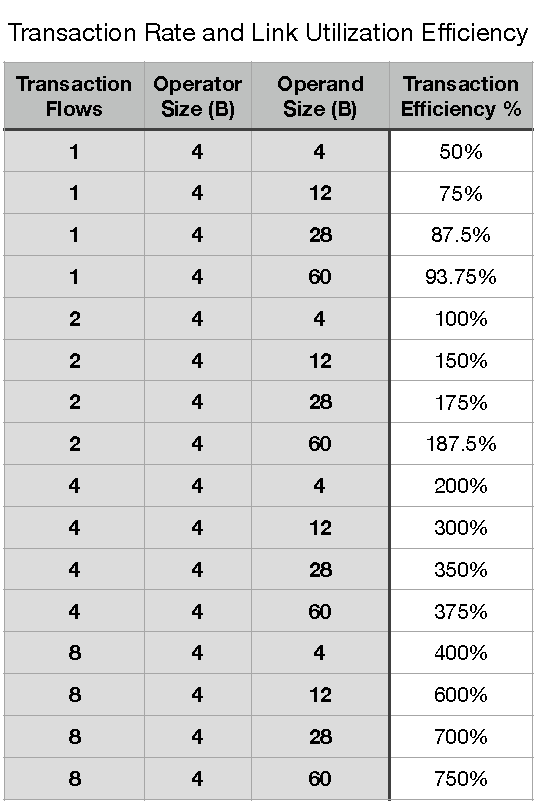
\includegraphics[width=0.92\linewidth]{.././figures/Transaction-Rate.pdf}
%  \caption{Transaction Rate Calculations}
%    \vspace{8pt}
%\end{marginfigure}



%\begin{marginfigure}
%        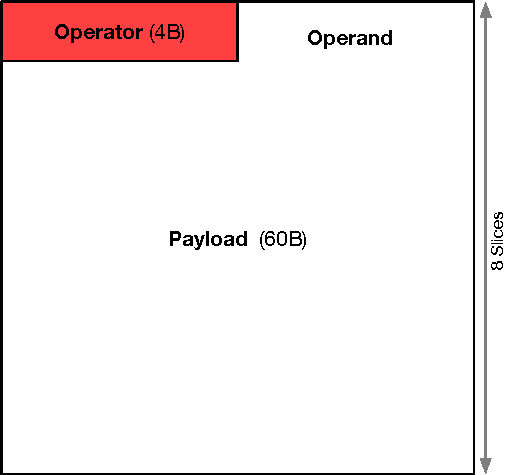
\includegraphics[width=\linewidth]{.././figures/8-slice-operator.pdf}
%  \caption{One 8 slice Flow Sub Transaction with 60B payload}
%\end{marginfigure}

%\subfile{Protocol-byte} % This is already included in the main file.

%
%\renewcommand{\bibfont}{\footnotesize}  % Footnote size for the whole bibliography
%\printbibliography

%\newpage
%\section{Virtual Channels}

%The protocol provides Endpoints for Virtual Channels. The IPV6 Format has been proposed, but this would give the false impression that the outside world (Internet) and inside world (Transaction Fabrix)/ %tm].trademark doesn't work

%\subfile{OPCODE-Byte}


